\chapter{Conclusion, Discussion and Future perspectives}
\thispagestyle{empty}
\emph{This final chapter first provides a short summary of the contents of the research findings, followed by a discussion of 
some of the relevant scientific issues that were addressed.}
\null
\vfill

\begin{myexampleblock}{Parts of this chapter are adapted from:}
  \authors{Caroline Durrant, Morris A. Swertz, Rudi Alberts, Danny Arends, ... , Ritsert C. Jansen, Klaus Schughart, et al}\\
  \emph{ Bioinformatics tools and database resources for systems genetics analysis in mice 
         - a short review and an evaluation of future needs}\\
  \bold{Briefings in Bioinformatics} (2011)\\\\
\end{myexampleblock}

\newpage

\section{General discussion}
This thesis advocates that using high-throughput computational methodologies and more optimised algorithms such as Pheno2Geno, 
or Multiple QTL mapping (MQM), combined with taking advantage of modern shared computational infrastructure, can provide a solution 
to the 'Big Data' challenges in Systems Genetics. Federated computing, and collaborative research, require tools such as the xQTL 
workbench, to work together and avoid duplicate efforts. This final chapter first provides a short summary of the contents of the 
research findings, followed by a discussion of some of the relevant scientific issues that were addressed. Also, conclusions are drawn 
on the impact of the Bioinformatics research and methodologies, presented in this thesis, on insights in Systems Genetics. The 
chapter concludes with an overview of future perspectives on research themes and methodologies in the interdisciplinary field of 
Systems Genetics and Bioinformatics.

\section{Highlight of the results}
Chapter \ref{chap:pheno2geno} details how Pheno2Geno was developed as R-package for the high-throughput generation of genetic markers and maps from molecular 
phenotypes. Pheno2Geno selects suitable phenotypes that show clear differential expression in the founders. It uses mixture modeling to 
select phenotypes showing segregation ratios close to the expected Mendelian segregation ratios, and transforms them into genetic 
markers that are suitable for map construction and/or saturation. Pheno2Geno analyses the candidate genetic markers and excludes those 
showing multiple QTL, epistatically interacting QTLs, and QTL by environment interactions, to provide a set of robust markers for 
QTL mapping and at the same time protecting against genetic markers from non-genetic origin.

Chapter \ref{chap:mqm} highlights the integration of the MQM algorithm into R/qtl. We validated the methodology with experimental data from a 
cross of A. thaliana Bayreuth x Shahdara. Sections \ref{sect:classical} and \ref{sect:Metabolites} show the performance of MQM on these experimental data. As the MQM 
algorithm is highly relevant to seed development, we discuss its use in this cross and try to find genetic factors underlying 
observed changes in the classical phenotypes and metabolome. We applied a generalised genetical genomics design \cite{Li:2009} to optimise the 
statistical power to detect QTLs and QTL x Environment interactions. This design approach allowed us to pick up more main effects 
and QTL x Environment interactions as compared to a random design or a full block design.

Chapter \ref{chap:ctlmapping} describes our current work on the topic concerning correlation differences when mapping two traits onto the genome. Our 
observations of the patterns when performing CTL mapping on multiple phenotypes, revealed that some of these patterns are similar 
to those when using a QTL x Environment interaction model. We applied this interaction model to data from a human Genome Wide 
Association Study (GWAS). We detected cell type specific eQTLs in whole blood for neutrophils, and show that low effect QTLs observed 
in samples can be explained by compensating for the relative number of neutrophils observed, or predicted. Cell type specific eQTL 
analysis will improve our power to detect QTLs and enables us to assign cell type labels to observed cis-eQTL effects.

Chapter \ref{chap:xqtlwormbench} details our work to provide computational infrastructure for the Life Sciences. We advocate the use of generators to 
create software and propose a generic and extensible data model (XGAP) \cite{Swertz:2010a} to store phenotype and genotype data. Combining these 
two approaches we developed several tools for 'Big Data' infrastructure. The combination of these tools is the xQTL workbench, 
a scalable web platform for the mapping of quantitative trait loci (QTLs) at multiple levels such as gene expression (eQTL), 
protein abundance (pQTL), metabolite abundance (mQTL), and phenotype (phQTL) data. Popular QTL mapping methods for model organism 
and human populations are accessible via the web user interface. The system also allows researchers to contribute new analytical 
routines. We conclude that good software infrastructure is of critical importance when scaling up large calculations to multi-core 
computers, clusters and cloud computing.

\section{Pheno2Geno performance}

Pheno2Geno is developed to optimise routines for generating genetics maps de-novo or to saturate existing genetic maps. Pheno2Geno enables 
the user to generate bio markers from microarrays, tilling arrays and RNA-sequencing data using mixture models \cite{Gort:2010}. Important design 
requirements for Pheno2Geno include being: 1) as generic as possible; 2) compatible to multi-core machines; and 3) to allow many machine 
clusters to generate genetic maps.

We developed Pheno2Geno to include a sensitive pre-selection of possible genetic markers with a simple t-test approach. This approach enables 
the user to quickly discard possible loci that do not show differential expression between parents. The method illustrates the trade-
off between the risk of missing important markers found by other approaches, and the time consuming computational burden of analysing 
all loci. Pheno2Geno was developed in the context that it is better to have a map in reasonable time, then not having a map at all.

We applied mixture models to select good genetic markers that show segregation frequencies comparable to the expected segregation 
frequencies \cite{West:2006, Truco:2013}. We demonstrated that our approach was much more generically applicable to finding genetic markers than the method 
proposed by Michelmore et al. (2006) \cite{West:2006}.

There are many tests to estimate a difference between two groups, including t-tests, linear models, mixture models etc. In a t-test 
only the mean values and variances are calculated. In our view, this provides the fastest way to decide if there is a difference. 
All other statistical methods mentioned above, come with added computational burdens such as ranking data or calculations that involve 
more statistics. The Pheno2Geno algorithm, however, is developed in such a way that is provides the user several other options for statistical 
testing (Wilcoxon Rank Testing, Mann-Whitney U Testing), and transformation of input signals (Log, Sqrt, Reciprocal, etc).

When creating maps for a Recombinant inbred line (RIL) (or a BackCross) population, in which case there is no parental information 
present, Pheno2Geno is still able to saturate a known low genetic map. Unlike other methods, Pheno2Geno does not require such parental information 
to detect the origins of the chromosomes. This is due to the fact that it flips anti-correlated chromosomes to find the optimal 
genetic map. A limitation of this procedure is that an initial genetic map has to be provided by the user.

The Pheno2Geno output structure is compatible with R/qtl \cite{Broman:2003, Arends:2010}. This facilitates an integrated experience between 
the map creation phase and the QTL mapping phase of the algorithm. Furthermore, when applicable function parameters were harmonised 
between the two software packages. Compatibility of the outcome structures of Pheno2Geno and R/qtl also provide further high throughput 
facilities for QTL mapping in inbred populations. With the upcoming new version of R/qtl (see section \ref{sect:limitations}) also the Pheno2Geno package will 
require updating to accommodate new specifications. The expected changes include: a standalone package, further optimisation of 
parallelisation, performance improvements, support for more crosses, e.g. diversity outbred and/or collaborative cross mice.

Taken together, the abovementioned features , i.e. pre-selection, generic software, optimised performance, R/qtl support, make Pheno2Geno a 
competitive package for genetic map creation in inbred populations. 

The Pheno2Geno algorithm also showed several drawbacks, which are discussed here. 

As a consequence of the pre-selection of possible markers, using Pheno2Geno may induce that certain markers are missed. This is due to the 
fact that we discard phenotypes based on parental expression, and not apply mixture modeling to all phenotypes. If mixture models 
would have been used to analyse all phenotypes, it is possible that more markers would have been detected.

Pheno2Geno currently does not support polyploid species such as corn, orchids and potato. For potato fitTetra was recently developed 
(Vosman et al. 2011 \cite{Voorrips:2011}). To create genetic maps of this polyploid species, it uses a comparable strategy to Pheno2Geno. It can be expected 
that future releases of Pheno2Geno will include support for these species, as the expertise for polyploid map creation is present in 
our group and the topic is subject of ongoing research. 

Pheno2Geno is written in R. Despite this computer language is frequently used in the analysis of biological data, it is also recognised 
that R is losing ground because of poor performance on extremely large datasets. We don't see this as a huge drawback because 
routines in Pheno2Geno are designed to minimise memory usage of the algorithm by providing 'lazy' equivalents of core functions, in such 
a way that data are only brought into RAM when necessary.

\section{MQM revisited}
The addition of MQM to the R/qtl toolbox has already shown to pay off in scientific terms: the paper that detailed the implementation 
has been cited more than 35 times since it was published in Bioinformatics in 2010 (Chapter \ref{sect:mqm}). This indicates how much the research 
community values a comprehensive multiple QTL mapping methodology integrated into an already well-established QTL mapping framework 
(R/qtl). Several applications of MQM are known to our group. For example, dr. E. Lodder (Academic Medical Center, University of 
Amsterdam, The Netherlands) used MQM to investigate collagen deposits in mouse left ventricular heart failure (publication in press). 
She discovered two additional loci which are of interest for further investigated as potential new therapeutic targets for cardiac 
interventions. In this thesis we also show two examples, concerning the classical phenotypes and metabolites in A. thaliana, in which 
we profiled MQM versus single marker mapping. Our analysis demonstrated that MQM detected more loci than the single marker mapping 
method, and the data showed more statistical confidence in the detected loci.

QTL mapping consists of two consecutive phases, modeling and mapping. In the modeling phase we look at the phenotype and assess the 
possible number of underlying QTL. We then use genetic loci to explain as much variation as possible. Subsequently, in the next phase 
of QTL mapping, the model is used and novel loci are included as assessed for their association with the phenotype of interest. We 
implemented multiple ways to build initial models for mapping analysis, including: forward model selection, backward elimination of 
cofactors from a full model, and the application of the user's own custom cofactor model. How precisely the different modeling 
techniques of MQM for systems genetics research are used, and their pitfalls, are described in a detailed 40 page manual.

We have chosen to merge MQM with the R/qtl toolkit, as it has already proven itself in the mouse QTL mapping community. It is generally 
viewed as the standard for QTL mapping in all inbred species, and provides a unified data structure on which algorithms work. This 
allows quick incorporation of new algorithms and provides a common basis for data exchange between researchers. 

MQM's core algorithm is written in C/C++ and is brought to R by creating a glue layer. Input to MQM is written in such a way that current 
R/qtl users can easily use the new MQM routine without need to reformat the data. However, because the code is mostly written in C/C++  
it is a trivial exercise to provide/interface MQM to different languages such as R, C/C++ and Ruby. This implies that the MQM routine is 
much more flexible to future changes in requirements or specifications, and/or language choice. It can also be extended to other tool 
boxes then R/qtl.

Earlier work has shown the following advantages of MQM for R/qtl to QTL mapping\cite{Jansen:1993, Handbook:Jansen:2007}: 

\begin{itemize}\itemsep1pt
\item Higher power, as long as the QTL explain a reasonable amount of variation.
\item Protection against over-fitting, because MQM fixes the residual variance from the full model, which allows the use of more cofactors than may be used in, for example, composite interval mapping \cite{Zeng:1994}.
\item Prevention of ghost QTL detection (between two QTL in coupling phase).
\item Detection of negating QTL (QTL in repulsion phase).
\item MQM gives (compared to CIM) a reduction in type I and II errors \cite{Handbook:Jansen:2007}.
\end{itemize}

The research in this thesis has added several other advantages, most notable:

\begin{itemize}\itemsep1pt
\item A pragmatic permutation strategy for controlling the false discovery rate (FDR) and prevention of locating false QTL hot 
spots, as discussed in Breitling et al \cite{Breitling:2008a}. Marker data are permuted, while keeping the correlation structure in the trait 
data. Because of the unified data structure in R/qtl, this permutation strategy can also be used with all other QTL mapping 
functions in R/qtl, such as single marker mapping and composite interval mapping (CIM).
\item High-performance computing by leveraging parallel computations using multi-CPU computers, as well as clustered computers, 
by calculating phenotypes in parallel, through the Message Passing Interface (MPI) of the SNOW package for R \cite{Tierney:2009}.
\item Visualisations for exploring interactions in a genomic circle plot (Fig. \ref{fig:circleplot}) and cis- and trans-regulation (Fig. \ref{fig:cistrans}).
\end{itemize}

The MQM for R/qtl also has drawbacks. It is computational much more intensive than single marker mapping. As it is designed in two languages, i.e. 
R and C/C++, the programme's maintenance is more difficult. Additionally, interpretation of the results is more complex when performing a multiple 
QTL scan. This is due to the fact that every phenotype is modelled in a unique way before scanning for QTL. 

\section{Visualising the output}
As stated above, using MQM may pose problems to the user/biologist, as the complexity of the model makes it much harder to interpret, as compared to 
the single marker QTL scan, which has a na\"ive model; one QTL for complex traits is by definition an oversimplification and (therefore) false. To 
alleviate the need for long and complex tabular output, we created circle plot visualisations (an example is shown in Fig \ref{fig:circleplot}). When 
scanning for interactions between multiple loci, it is common to compare everything versus everything. Since MQM provides us with a model of the main 
effect loci, we are able to quickly assess any interactions between them because we only have to analyse a hand full of possible interactions, i.e. 
between main effects. This allows us to quickly build up the circle plot with main QTL effects as well as interactions, which cannot be done for a 
single marker scan as no such model is present. 

This type of visualisation provides researchers:

\begin{itemize}\itemsep1pt
\item Output per trait: an overview of interesting genetic loci (main effects) and the interactions between these main effect loci.
\item A holistic overview of all traits to identify co-localisation of main effect QTLs on the genome.
\end{itemize}

Furthermore, we added cis and trans visualisations which allow the same data to be explored in a 2D fashion providing comparable information to the 
holistic overview circle plot. Circle plots show the main effects and the interactions between genetic loci for a single phenotype, while cis/trans 
plots show main effects for many phenotypes, combined with genetic location information of the (expression) phenotypes mapped. 

\section{Limitations of R as analysis platform for R/qtl}
\label{sect:limitations}
When dealing with high throughput data obtained from RNA-seq, exome sequencing or Bisulphite sequencing, data size quickly becomes the limiting 
factor for software written in R \cite{Ristić:2009, Patel:2012}. Because R/qtl-HD is aimed at QTL analysis of high-density, high-throughput data, R is not a suitable language 
for the high throughput computational parts of the algorithms. R/qtl-HD is written in the high performance D programming language. D is chosen 
as primary language because it was developed to perform safe and high throughput numerical analyses. D uses a C like syntax \cite{Alexandrescu:2011}, and therefore 
provides a familiar syntax to the R/qtl developers, most of whom have a C/C++ background, making D the language of choice for R/qtl-HD. 
Additional features of D include:

\begin{enumerate}\itemsep1pt
\item \emph{Improved code quality} - This increases options for maintenance of the code. Also, a more readable code is more open to discussion and reasoning 
to optimise the code, which results in improved performance of the algorithms.
\item \emph{C ABI compatble} - D allows to call C. D directly allows to call C functions and a limited subset of C++. This allows to re-use previously written R/qtl code 
(written in R and C) \cite{RQTLGuide:2009}.
\item \emph{Built-in unit testing} - Unit testing is built into the D programming language, which facilitates programmers to use the power of unit- and 
regression testing to build a test suite without the need for external tools or frameworks.
\item \emph{Concurrency and Actors} - The D language provides high level patterns such as Actors and Message Passing to deal with parallelisation of code. 
Unlike other languages, this is a built in feature of the language, which allows the standard D library to use safe lock free concurrency mechanisms \cite{Alexandrescu:2011}.
\item \emph{Static typing} - D requires types (e.g. Integer, Float, Double) to be declared and known at compile time. This improves readability of the code 
and reduces the risk for run-time type errors of the system.
\item \emph{Compile Time Function Execution (CTFE)} - CTFE is a feature that allows to build look up tables at compile time. This greatly reduces the run 
time of algorithms, by pre-calculating common cases \cite{ArendsBlog:2012}.
\end{enumerate}

These are the main reasons for the R/qtl development team to favour D over R. The current version of R/qtl provides many tools for genetic map 
construction, but also several historic methods for QTL mapping. R/qtl-HD will not provide a multitude of methods but focuses more on the high 
speed analysis of data using stable and proven methods such as Haley-Knott regression \cite{Haley:1992} and analysis of variance. Additional features such 
as genetic map construction and validation are not high priority when converting the R/qtl software into a more optimised language. R/qtl-HD 
is designed for mapping huge volumes of phenotypes onto medium to large genetic maps \cite{Trelles:2011}.

Furthermore MQM from R/qtl will also be converted into the D programming language. The MQM routine has proven to be a useful addition to the R/qtl 
toolkit and with the new implementation of R/qtl as R/qtl-HD, we aim to improve its usefulness even more. The major limitation in MQM is the additional 
computational load when compared to single marker QTL mapping \cite{Arends:2010}. The R/qtl development team is committed to: 1) add the MQM routine to the 
R/qtl-HD package, and 2) provide further optimisation to MQM allowing it to handle even larger volumes of phenotype and genetic data.

\section{CTL \& Cell type specific eQTL}
Presently, more and more research is being done to understand eQTLs and their effects on phenotypes. Recent papers reported the detection of some sex 
specific eQTLs \cite{Ramos:1999, Bernatchez:2008, Lusis:2010}, as they were present in females but not in males, or vice versa. Sex is obviously not 
the only covariate that can be used in these QTL x Environment analyses; other possible covariates are population structure, age, and cell type. Our 
findings thus indicate the need to add cell type specific covariates in QTL mapping. One of the main advantages of using cell type as covariate is 
that we can compartmentalise environmental variation. This allows easier detection of associations between genetic loci and observed differences in 
phenotype, because some of the variation from non-genetic origin has been captured by the cell type covariate.

This method of mapping QTL x Environment interactions is not new, although in our studies we applied it to cell types. However, this procedure was 
complicated by the fact that cell type abundance was only measured in two cohorts. The available cell counts were: lymphocyte, neutrophil, and RBC 
counts/percentages. As we used six cohorts in total, we had to infer the cell counts for the remaining four cohorts. Using the predicted cell counts 
in these four cohorts, we were now able to perform our eQTL meta-analysis. This approach to handling cell type (for an eQTL) is similar to dealing 
with an environmental factor. When using a basic interaction model, combined with cell type percentages, we can clearly distinguish between eQTLs 
which seem to be neutrophil specific and lymphocyte specific.

Large sample sizes are required to perform such interaction analyses with reasonable power to detect interaction effects. Currently, we can only 
obtain the required sample sizes by using meta-analysis of multiple eQTL GWA studies. The meta-analysis method increases our sample size dramatically 
as compared to a normal GWAS. This increase in sample size allows us to detect more eQTL, but is also helps to reduce false positive eQTLs. Furthermore, 
we can use an additional level of information to assess our eQTLs. Looking at the direction of the eQTL effect in different cohorts, allows assessment 
of the consistency of the direction across multiple datasets. 

Known genetic variants underlying for example Crohn's disease, IBD (inflammatory bowel disease) or asthma, are available from the literature 
\cite{Hindorff:2009}. In our study we demonstrated that using meta-analysis allows to assign cell type labels to all eQTL detected. Combining 
these two sources of information allows us to test if the eQTLs showing association with a disease (such as Crohn's disease) are specific for a 
certain cell type. This information can be used in future research to find therapeutic targets for these diseases, or to understand why certain 
targets which might seem valid at first, turn out not to be effective.

Our study revealed that Crohn's disease indeed has a strong neutrophil component ($P < 0.0018$). While Crohn's disease showed a significant number of 
neutrophil specific eQTL, this was not the case for IBD. We conclude that derangements in different cell types are involved in IDB and Crohn's disease. 
This is surprising, because Crohn's disease is classified as a type of IBD \cite{Sandborn:2012}. Here we find supporting evidence that different 
pathophysiological processes are present in Crohn's disease, as compared to other IBD conditions such as Colitis ulcerosa. 

The methodology for cell type specific eQTL also revealed some disadvantages. The selection of the covariate is very important. Here we used a 
continuous variable (cell abundance or cell percentage), in a comparable way to the mapping of sex specific eQTL, where the covariate is a 
dichotomous variable (male or female). As a consequence, in practice it is much harder to detect sex specific eQTL, as compared to cell type-eQTL. 
We assume this is the reason why so few sex specific eQTLs are reported in the literature.

Another aspect is that large sample sizes are required for analysis. Methodological issues concerning meta-analysis include the usage of multiple 
platforms (Illumina \& Affymetrix) and even multiple versions from the same manufacturer (e.g. Illumina HT8, HT12). All this data needs to be 
integrated in a comprehensive and precise way.  This creates a need for good infrastructure to keep track of the differences between data sets, 
and analytical tools which can handle missing or incomplete data \cite{Trelles:2011, Prins:2012}.

Several disadvantages arise in the context of experimental realities. Cell types are hard to purify and identify. In our opinion it is impossible 
to acquire a 100\% pure fraction of, for example, CD4 T-Helper cells. Despite this, our method assumes that we can identify cell types without 
much bias. This might not be the case for some cell types which are present in many distinct sub cell types (such as T-cells), and consequently 
we cannot distinguish between them. Another example of a problematic situation refers to the changing expression patterns of harvested and purified 
neutrophils. These patterns may differ largely from the patterns when the neutrophils are still circulating in the blood.

\section{xQTL workbench for infrastructural issues}
The need for reliable and flexible infrastructure in Systems genetics sparked our interest to develop the xQTL workbench. It combines the flexibility 
of the MOLGENIS generator suite \cite{Swertz:2004} with the most frequently used computational and analytical tools for Systems genetics (i.e. R/qtl 
\cite{Broman:2003, Arends:2010}, Plink \cite{Purcell:2007} and many other tools). Using R as Esperanto between the different languages creates a system 
for systems geneticists to keep track of data generation and their analyses. Additionally, using R as computational back end allows researchers to 
contribute their methods and algorithms back to the scientific community by uploading them into the xQTL workbench. While the xQTL workbench system 
described in this thesis has the ability to absorb new analytical methods, we also considered the need for high flexibility. We expect it will be 
difficult to anticipate to new demands, requirements or new developments, that could offer better alternatives than databases for data and R for 
analysis \cite{R:2005}. Despite this, in our opinion the xQTL workbench is well suited to tackle such changing requirements by leveraging the strength of 
generators and the flexibility of the XGAP data model.

Infrastructure in Systems genetics is created with generators, as it alleviates the need to handwrite most of the system's common codes \cite{Swertz:2004}. This common 
code consists of basic database parts such as: Create, Read, and Update functions for the underlying database system, generated web interfaces to enter 
and curate data, and application programming interfaces (APIs) \cite{Swertz:2010b} to transfer data from one language (e.g. Java) to another (e.g. R). We used the MOLGENIS 
generator together with the flexible XGAP data model \cite{Swertz:2010a} to set up a system capable of handling any genetical genomics experiment 'at the push of a button' 
as the unofficial slogan states. All our collaborators reported gains on implementation time when using the xQTL workbench, as compared to a handwritten 
system in which all these components need to be (re)developed or invented. Parts of the system will always require fine tuning, but major parts of 
functionality do not change from one database system to the other, and thus allow automated generation of these parts.

The xQTL workbench allows R code to automagically use Cluster and Cloud computing for trivial parallelisable algorithms. An example of this is QTL mapping 
in which every phenotype is analysed independently. With a multi core machine the distribution of computations to separate CPUs is easily achieved without 
much overhead (such as network latency). When using the xQTL workbench, researchers are able to write algorithms suited for a single 
phenotype/marker/individual, and test their analysis on their local desktop. When the algorithm is completed the developer uploads the new algorithm into 
the xQTL workbench and applies it across rows/columns of the stored matrices. The user can then choose to use any available backend (either local host, 
Cluster or Cloud) to perform his/her computations. The xQTL workbench deals with distributing computations (if the analysis supports distributed computing) 
to multiple nodes when applicable. 

An ever increasing amount of data and knowledge (in terms of the outcomes of computational analyses) are stored in large databases and are available to 
biologists for further study. This allows reuse of data by different biologists, decreases the need to regenerate data, and it stimulates collaborations 
between research groups. Furthermore, translational databases (e.g. NCBI DB-GAP \cite{Mailman:2007}, KEGG \cite{Goto:2000}), which store and integrate 
data across many species, facilitate interactions between research communities, such as Human and Worm genetics, by providing an opportunity to look 
across the borders of their own species \cite{vanDerVelde:2014}. 

At the same time, storage of raw data is still necessary in many cases. A good example is found in the next generation sequencing platforms. Although the 
costs for sequencing are being reduced in a high pace, additional funds are required to store and process the raw data coming from the machine. While at 
the one hand costs of sequencing are dropping, at the other hand sequencing produces more data as the technique is being performed at small hospitals and 
large sequencing facilities. It can be expected that when the price of sequencing becomes low enough, i.e. the costs of re-sequencing drop below the 
costs of storage, storage of raw data will probably be replaced by storage of samples (which are also stored now for re-analysis/validation). Such 
developments are likely to decrease the immediate need for storage space, but increase the computational burden of sequencing.

In this thesis we advocate R \cite{R:2005} as Esperanto language between storage and computational parts of our xQTL workbench platform. Our choice for 
R is motivated by several reasons including: 

\begin{enumerate}\itemsep1pt
\item MOLGENIS provides a generated R API, that we used to plug in our analysis tools.
\item Many analytical tools are already available for R.
\item Biologists tend to be familiar with R, since the language is frequently used in data analysis. As a consequence, they can share their analysis software through the system.
\item R provides built in support for web browsing and secure connection (using Rcurl).
\item R provides an easy way to start/stop shell scripts.
\end{enumerate}

Despite the realisation that other languages also fulfil (most of) these requirements, our familiarity and experience with R largely 
contributed to the decision to build the system with these components.

Application examples of the xQTL workbench system are the wormQTL \cite{Snoek:2012}, and the wormQTL-HD \cite{vanDerVelde:2014} databases. These databases 
contain a lot of worm data and provide the worm research community with tools for analysis. The wormQTL-HD database comes with the added advantage that 
it couples the worm phenotypes to human phenotypes. Consequently, geneticists working in the human domain can search for non-obvious (worm)-models to test 
their hypothesis in worm. In other words, the database functions to bring these research communities closer together.

Several issues are relevant to consider in terms of disadvantages of the xQTL workbench. It is a complex system to set up for biologists, as its software 
is used as basis and requires other infrastructure on top. Therefore, programmers with knowledge of R, Java, and Unix are required for setting up the 
system and facilitate its maximal use.

Furthermore, the xQTL workbench system only provides several QTL mapping routines that are available as proof of principle. Further adaptation of the 
system will increase the number of tools available in the workbench. While not a major disadvantage, it implies, for example, that MQM is not yet 
available to the users although it can easily be added and implemented into the system.

Using a generator requires regular updates. In doing so, introduces the risk to break the code in many (generated) places. A full and extensive test 
suite is then required to test the generated parts of the software for consistency and stability. Weighing the pros and cons, we consider this not 
really a drawback because a full test suit also raises confidence in the software, and makes it more reliable. 

\section{Applications in Biology}
The final research question of this thesis refers to the impact of our contributions and developments  in the field of Bioinformatics on advancements 
in methodology and knowledge in Systems genetics. During the research project we regularly tested our tools and performed various experiments to 
validate our computational approaches. 

In this thesis we show the application of Pheno2Geno on a large dataset containing expression data from tilling arrays. Tilling arrays are a sensitive way to 
measure genome wide expression levels of RNA transcripts. They produce a large amount of data. Pheno2Geno uses these expression data to generate new high 
quality maps for QTL mapping, thereby exploiting the availability of QTL information in high throughput phenotypes. We obtained raw expression data from 
our collaborators at Wageningen University (RAW 16.8 GB) and were able to analyse these data in less than 30 minutes on an average workstation. Genetic 
maps obtained were then used by the researchers to improve the resolution of their subsequent eQTL mapping. The observed increase in resolution allows 
the detection of leads in smaller regions of interest, and lowers costs for follow up analyses of the traits of interest.

Application of MQM has identified new genetic loci of interest in different studies. The benefits are thus more insight in the underlying genetics. 
This leads to an increase in knowledge about how to improve pathways for production of commercially interesting biological or therapeutic substances 
or products. Furthermore, by increasing the amount of loci detected MQM (as well as cell type specific eQTL mapping) we are able to better understand 
the genetic basis of heritable traits, such as crop yield, seed quality, and disease susceptibility, for example Crohn's disease. MQM improves our 
statistical model by adding genetic loci as explanatory variables, while cell type specific eQTL mapping does this by incorporating environmental 
effects. Although we only applied our cell type specific eQTL mapping to neutrophils and lymphocytes in whole blood as proof of principle, we 
observed that SNPs associated with Crohn's disease are present more often than randomly expected to show a neutrophil specific eQTL effect.

Our system xQTL workbench was used as storage and computation platform in wormQTL and wormQTL-HD databases. Furthermore an Arabidopsis database is 
presently being developed to contain similar features as the womQTL database. We demonstrated the need for translation analysis in wormQTL-HD and 
connected worm and human data. This shows (and confirms findings from other studies) that worms can be used as model organism to test in worms certain 
hypotheses derived from observations in humans. The advantages provided by the xQTL workbench allow other researchers to accomplish the same aim: 
storage of large amounts of data and performing reliable/traceable analyses while avoiding duplication of efforts.

An illustrative example is the following. When I started my PHD research in 2009, my largest dataset was 100mb (24 mice measured on 30k probe 
microarrays). This was easily manageable on a single computer and involved no storage or computational issues. Just four years later we cannot 
perform the same analysis because the size of the data obtained from the same experiment has increased so much, that a database that can handle 
many gigabytes is required. Such an amount of data can only be stored using dedicated hardware, which also stores the complex relationships 
between the data. To allow integration of information from worms and humans in less than a minute, computations need to be optimised and 
distributed across many nodes of a cluster. The knowledge gain of this high throughput data is that biologists are able to develop new 
hypothesis while browsing data collected by hundreds of people over a time scale of decades. 

\section{Future perspectives}
As the interesting and novel developments are created at the interface of the research fields of Systems genetics and Bioinformatics, this 
section first looks into the future of both fields separately, after which some ideas about the interdisciplinary domain are presented.  

Genetics research is producing more data than ever before. This leads to an almost exponential increase in data similar to Moore's law of 
computing, which states that '\emph{Every 12 to 24 months CPU power doubles}' \cite{Moore:1975, Moore:1998, Editorial:2009}. Large scale sequencing facilities such as the Sanger Institute (USA) and 
the Beijing Genomics Institute (China) continue to produce an ever increasing stream of sequencing data for still increasing costs per 
analysis. This allows researchers to collect data on an unprecedented scale, but also triggers the massive re-use of previous data.  

The field of epigenetics is also gaining more and more attention, in particular the field of DNA methylation. The creation of epiRILs \cite{Johannes:2011} means 
that we have a genetic map to associate our phenotype with, but additionally we can look for epigenetic inheritance of phenotypes using an 
epigenetic map. This seems trivial, but in fact it describes the easiest situation which already doubles the required amount of effort for 
mapping QTLs, because we need to map to a genetic map and an epigenetic map. Furthermore, epigenetic map currently available only shows the 
inheritance of stable epigenetic states in an experimental population without any sequence variation. Therefore, the situation is even more 
complex in the case of natural populations which have a mixture of genetic and epigenetic variations \cite{Johannes:2014}. At present the 
stability of Epigenetics is still uncertain and it may lead to a reconsideration of certain genetic theories, in particular those addressing 
the inheritance of DNA. This daunting challenge of first understanding how epigenetics play its role in inheritance, and then using this 
knowledge to improve our QTL mapping ability will be a major and exciting challenge in the coming years.

Cell type specific eQTLs are just one of many possible interaction models to take into account during eQTL mapping. The current trend of 
performing data driven research in which we increase the amounts of data being collected and connect everything with everything is expected 
to remain in the future. The statistical downside is that it causes multiple testing issues \cite{Benjamini:2010}, population stratification issues, and 
spurious associations by hidden factors \cite{Huff:1993} and/or batch effects. 

The field of Bioinformatics faces the computational challenges arising from the above trends and expected developments. The question is how we 
can contribute to solve these issues, demonstrate the added value of our applications, and present our legacy for the coming years.

Computational power has always increased exponentially over time. Recently, however, the Intel Company announced that Moore's law is not valid 
anymore \cite{Editorial:2009, Shah:2013}, and last 3 years and the upcoming years will show a less then exponential growth in power per CPU \cite{Shah:2013}. It can be expected 
that the production of new and cheap computers will slightly offset this problem. Therefore, while separate CPUs will fail to show exponential 
increases in speed, another development is the emergence of new and improved dedicated machines, such as ARM cores, Field Programmable Gate 
Arrays, and ASICS miners for dedicated computation. Although these machines are less or equally powerful in general, they are designed to excel 
in just one specific task, compared to a CPU which does many different tasks. Our research showed that several 'smart' algorithms, of which some 
could be hard coded into an ARM core or FPGA, allows the same computations to be executed much faster compared to a CPU. Taken together, this 
will still allow scaling up, for example of cell type specific eQTL analysis, to even larger data sizes.

We advocate using linear scaling of multicore machines or large compute clusters. Although this is not the solution to our problems, using these 
systems such that data are presented in a summarised way to biologists (as is done by wormQTL) will help to relieve some of the immediate need 
of collaborators. In our opinion the xQTL workbench will continuously be developed to suit emerging new technologies in the field of data storage 
and computation. Additionally, using R as Esparanto between multiple languages means we are less dependent on a single language, and are able to 
switch from one storage strategy to another, while the computational part of the system does not 'see' this change because it only sees the R 
glue layer.

The computational issues arising from high throughput data can be partly solved with smarter algorithms such as Pheno2Geno, MQM, CTL and cell type eQTL. 
Some of these algorithms (Pheno2Geno, MQM, cell type eQTL) are already being used actively in research, and show that improved tools give either improved 
performance or improved power to detect results. 

The xQTL workbench is a collaborative system in which bioinformaticians and biologists contribute to create a system which can serve both them and 
the communities to which they belong. Collaborators are curating data and adding new analysis routines to the wormQTL system. Pheno2Geno connects to R/qtl 
but we expect other QTL mapping packages without map creation facilities to be also interested to add Pheno2Geno to their pipeline. Additionally the 
whole high throughput eQTL mapping pipeline is available for other researchers to use and learn from. We urge all people performing GWAS to perform 
meta-analysis (when possible) to improve their results and employ a strategy such as cell type specific eQTL mapping. 

How and where do Bioinformatics and Systems Genetics come together? High throughput data is the connecting factor between both fields. Systems 
genetics cannot exist without the help of high throughput methodologies such as whole genome sequencing and automated proteomics, because only 
with these technologies we are able to build a comprehensive picture of all the bio-molecular levels that compose organisms. To generate 
biologically relevant knowledge from these large amounts of data, geneticists cannot do without bioinformaticians. 

Here we have shown our contributions to the field of bioinformatics such as novel infrastructure, high-throughput computational methodologies and 
more optimised algorithms. These advances aid faster data processing, reduce redundancy during analysis, and create novel tools to get more out 
of existing data. New tools and improvements of existing tools, as presented in this thesis, combined with computational advances, creates the 
opportunity to do new things which were not possible before, such as large scale cell type specific eQTL mapping on 6000+ human GWAS samples. Our 
tools will help Systems geneticists to do their job better and in less time than before.  

\chapter{Additional for Dissertation}
\thispagestyle{empty}
\emph{This additional chapter containing some additional sections, such as a Dutch summary, 
list of abbreviation, etc, needed for a complete dissertation required for a promotion at 
the University of Groningen.}
\null
\vfill
\newpage

\section{Dutch Summary / Nederlandse Samenvatting}
Systeem genetica is een inter disciplinair veld wat zich bezig houdt met de gevolgen van 
genetische variatie op alle bio moleculaire niveaus een biologisch systeem. Het effect van 
deze genetische variantie leidt tot verschillen in fenotypen, zoals opbrengt en resistentie. 
Het doel van systeem genetica is het indelen van de oorzaken van deze geobserveerde 
fenotypische variatie in drie categorie\"en: Genetische effecten, omgevings-effecten en 
(random) residuele error variantie. Door netwerken te bouwen van interacties tussen 
alle bio moleculaire niveaus probeert systeem genetica complexe fenotypen te verklaren uit 
het samenspel tussen deze niveaus.

Biologie gebruikt natuurlijke variatie en genetische perturbatie om de componenten te ontrafelen
die fenotypische variatie veroorzaken op verscheidene bio moleculaire niveaus zoals: genetica, 
transcriptomics, proteomics en metabolomics. Bio moleculaire metingen gecombineerd met pertubatie 
van verschillende omgevingsfactoren stellen ons in staat om de invloed van verschillende 
effecten zoals omgeving en omgeving x genotype te bepalen. Experimenteel ontwerp en statistiek 
worden gebruikt om error variantie te minimaliseren.

Moderne high-throughput technieken genereren grote hoeveelheden genomische, transcriptomic, proteomic 
en metabolomic data. Een enorme uitdaging voor bioinformatica zit in de omvang van de data die verzameld 
wordt en de diversheid aan technieken die worden gebruikt. Deze thesis zal ingaan op onze oplossingen 
voor deze 'Big Data' uitdaging binnen de systeem genetica. Deze thesis adviseerd om geoptimaliseerde 
algorithmes te gebruiken zoals: Pheno2Geno of Multiple QTL mapping. We promoten verder een collaboratieve 
aanpak voor data opslag en gerelateerde computationele aspecten (xQTL workbench) om high throughput data 
op te slaan en te analyseren binnen de systeem genetica.

Hoofdstuk \ref{chap:introduction} bevat een korte historische introductie over systeem genetica, 
In de volgende hoofdstukken van deze thesis laten de bijdrages zien van deze thesis aan systeem genetica.

Hoofdstuk \ref{chap:pheno2geno} (Pheno2Geno) gaat over het construeren van genetische kaarten vanuit grootschalige 
omics datasets. De theorie achter het maken van genetische kaarten is ongeveer 100 jaar oud. Maar 
software beschikbaar voor het maken van genetische kaarten in model organismes is nog 
vaak nog niet aangepast aan nieuwe ontwikkelingen zoals multicore computers en cluster computing. 
Pheno2Geno is software voor het maken van genetische kaarten uit Big Data verkregen door 
experimenten de gebruik maken van tilling arrays of RNA sequence experimenten.

Hoofdstuk \ref{chap:mqm} omschrijft de implementatie van het multiple QTL mapping algoritme 
in R/qtl. Hiermee voegen we een nieuw algoritme aan de R/qtl toolset toe, een 
toolset speciaal ontwikkeld voor het mappen van QTLs in ingeteelde (muis) populaties. R/qtl 
vormt de basis van meerdere tools die allemaal gebouwd zijn rond een gedeelde datastructuur. 
Deze structuur maakt het makkelijk om software aan te passen en nieuwe tools toe te voegen.
Door de vele tools, kunnen onderzoekers snel wisselen van methode wanneer dit vereist is of 
verschillende methodes vergelijken zonder een nieuw software pakket te hoeven leren.

Huidige werkzaamheden over het gebruik van \emph{verschillen in correlatie} om interactie 
netwerken te genereren en celtype specifieke eQTL effecten op te sporen wordt beschreven in 
hoofdstuk \ref{chap:ctlmapping}. Correlated Traits Locus analyse (of CTL mapping) laat 
onderzoekers toe om genetische loci te vinden die geassocieerd zijn met correlatie verschillen 
tussen segregerende fenotypen. Een variant op deze methode is waardevol gebleken om cel 
type specifieke expressie QTL (eQTL) effecten te ontdekken. Deze effecten kunnen worden 
gebruikt om mengsels van cellen te ontwarren. We passen onze nieuwe methode toe op een cel 
mengsel van geheel bloed gen expressie data en laten zien dat we in staat zijn om cell type 
specifieke eQTLs te detecteren.

In hoofdstuk \ref{chap:xqtlwormbench} presenteren we onze idee\"en voor een generiek opslag en rekenplatform 
voor systeem genetica. Ons demo systeem xQTL workbench wordt momenteel gebruikt als een 
backend voor de WormQTL en WormQTL-HD databases. In xQTL workbench kunnen gebruikers hun 
gegevens op slaan en delen in een lokale of webomgeving, en lopen analyse over datasets met 
behulp van de kracht van gedistribueerde computing. Het wordt standaard geleverd met QTL 
mapping tools, zoals: R/QTL, Plink en qtlbim maar ook biedt het een web inferface, data 
importers, API's en visualisaties.

Ik vertrouw erop dat je geniet van het lezen van dit proefschrift, zoals ik heb genoten van het maken 
ervan.

\newpage
\section{Abbreviations and Acronyms}
{\footnotesize
\begin{tabular}{ l l }
API:         & Application Programming Interface\\
BC:          & Backcross \\
bp:          & Base pair(s) \\
cM:          & centi Morgan \\
CIM:         & Composite interval mapping \\
CPNN:        & Collaborative computing project for NMR\\
CSV:         & Comma separated values\\
CTL:         & Correlated traits locus \\
DesignGG:    & Experimental design of genetical genomics software\\
DRY:         & Principle of don't repeat yourself\\
DSL:         & Domain Specific Language\\
EBI:         & European Bioinformatics Institute\\
FINDIS:      & Finish disease database\\
GEMs:        & Gene expression based genetic marker\\
GEN2PHEN:    & EU project to unify human and model organism genetic variation databases\\
GMOD:        & Generic model organism database project\\
GUI:         & Graphical user interface\\
GWAS:        & Genome Wide Association Study\\
GWL:         & Genome Wide Linkage analysis\\
HGVBaseG2P:  & Human genome variation database of genotype-to-phenotype information\\
HTML:        & Hypertext markup language\\
IDE:         & Integrated Development Environment\\
JAR:         & Java Software Archive\\
LGPL:        & Lesser general public license\\
MAGE-TAB:    & Microarray gene expression tab delimited file format\\
Mbp:         & Mega base pairs = 1.000.000 bp \\
MOLGENIS:    & Molecular genetics information systems toolkit\\
NordicDB:    & Nordic Control Cohort Database\\
OBF:         & Open Bioinformatics Foundation\\
OntoCAT:     & Ontology common API toolkit\\
PEAA:        & Patterns for enterprise application architecture\\
QTL:         & Quantitative trait locus\\
RDF:         & Resource description format\\
REST:        & Representative state transfer web services\\
RIL:         & Recombinant inbred line \\
SNP:         & Single Nucleotide Polymorphism\\
SOAP:        & Simple Object Access Protocol\\
SQL:         & Structured Query Language\\
UML:         & Uniform data Modeling Language\\
WAR:         & Web Application aRchive file\\
XML:         & Extensible Markup Language\\
XGAP:        & Extensible genotype and phenotype software platform. 
\end{tabular}
}
\newpage

\section{Acknowledgements}
Knowledge is in the end based on acknowledgement\\
- Ludwig Wittgenstein (1889 - 1951)\\\\

There are many people who need to be thanked and acknowledged, 
here are the people who made the cut:

{\bf Ritsert C. Jansen} to whom I owe my life in science, thank you for giving me this chance 
to work in your group and develop my skills in research and education. {\bf Anna Mulder}, my 
girlfriend, for all the times I left you and {\bf Oscar} (our cat) for my science endavours. 
Thank you for your trust in me and giving me a home to come home to.
My family {\bf Bert}, {\bf Dinie}, {\bf Johan} and {\bf Jos\'{e}} for their support and understanding. 

{\bf Pjotr Prins} Always forgotten, Never Ignored. 

I would like to thank all the people past and present at the {\bf Groningen BioInformatics Centre} 
(GBIC) group for putting up with me. In particular, {\bf Yang Li} for your mentorship and all the 
vibrant discussions we had at GBIC and {\bf Joeri van der Velde} my friend and coworker for the 
good times hacking on Java and R in Haren.

{\bf Morris Swertz} my co-promotor, you were a great help when writing chapter \ref{chap:xqtlwormbench} 
and always made me feel at home at GCC. Also all the guys from the {\bf Genomics Coordination 
Centre} (GCC) department for all the presentations, discussions, coffee served by {\bf Roan Kanninga} and 'end of sprint' beers. 
{\bf Frank Johannes}, {\bf Gerard te Meerman} and {\bf Martijn Dijkstra} for pre reading this thesis and proving me 
with feedback and suggestions. Additionally I would like to thank everyone from {\bf JohannesLab} for participating during Tuesday morning 
seminars and journal clubs. 

{\bf Lude Franke} and {\bf Harm-Jan Westra} for the very informative collaboration on the 
human GWA study (chapter \ref{sec:cellspecificeqtl}), I learned a LOT from you, and am 
extremely thankful for your help with the final chapters of this thesis. 

I have been very lucky to meet and work together with some of the cleverest minds in animal breeding 
and genetics. Being able to discuss my ideas with people such as {\bf Karl Broman}, {\bf Gary Churchill}, 
{\bf Allen Attie} and {\bf Brian Yandell} made me push myself to the limits and beyond. I would like 
to thank all of you for the nice times I had across the pacific ocean. 
Additionally I was lucky to have good collaboration with Wageningen University, especially {\bf Wilko 
Ligterink}, {\bf Henk Hilhort} and {\bf Ronny Joosen} for doing the \emph{Arabidopsis thaliana} 
experiments, and trusted me to analyze their data. I learned a lot especially about the more 'biological' 
parts of this thesis. 

Furthermore I have had the pleasure to work with many dedicated students along the way: 
My student {\bf Konrad Zych} for his dedication and help with Pheno2Geno and chapter \ref{chap:pheno2geno}. 
{\bf Mark de Haan} for his work on the xQTL workbench system and the review work on Pheno2Geno.
{\bf Yalan Bi} for working on the \emph{A. thaliana} gene expression data and alternative splicing 
work, which unfortunately was not finished in time for this thesis. And {\bf Adriaan van der Graaf} for 
showing me that even jocks can be turned into nerds. And naturally all the other students I have been 
privileged to work with during these last years.

I would like to thank the {\bf European Union} for setting up the {\bf SysGeNet} network, I've met 
many people and learned a lot about the mouse community in Europe. Especially I would like to thank 
{\bf Klaus Schughart} for starting and maintaining the network, and {\bf Leonard Schalkwyk} for 
inviting me to the UK for a lecture series at King's College.

{\bf Richard Stremme} and {\bf Evert van der Velde} for always being available after work for a beer and providing
entertainment and the needed distraction when being fed up with writing this thesis.
The {\bf University of Groningen} (RUG) for educating me and providing me with an place to do my research. And 
finally the {\bf University Medical Centre Groningen} (UMCG) for the pleasant working atmosphere and good lunches.

\newpage

\section{About the author}
\subsection{Curriculum Vitae}

\begin{wrapfigure}{r}{0.4\textwidth}
  \centering
  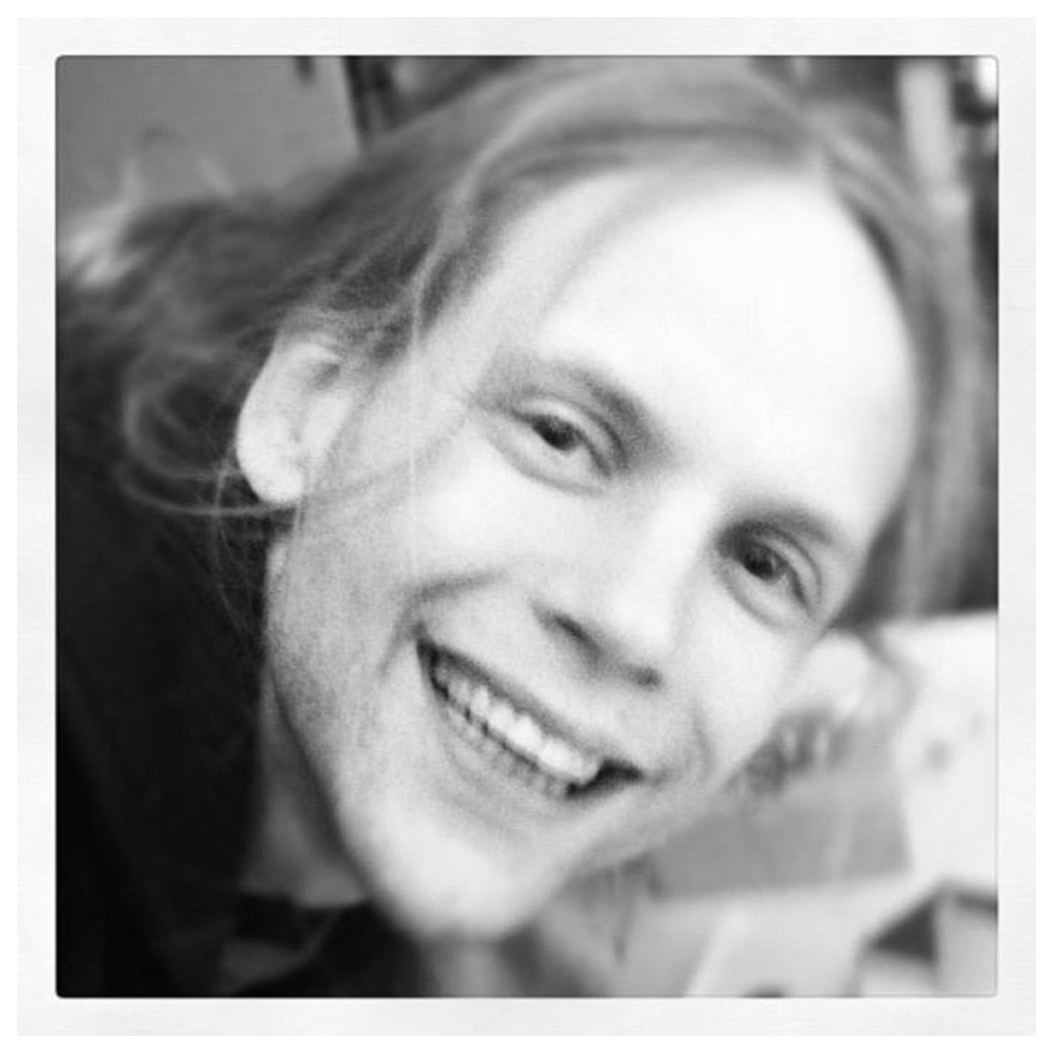
\includegraphics[width=0.3\textwidth]{eps/image_6_1.eps}
\end{wrapfigure}

Danny Arends was born on the 15th of Juli 1983 in the city of Zwolle located in the heart 
of the Netherlands. After moving twice, Danny went to an elementary school situated in 
Heiligerlee, a minuscule hamlet in the north of Holland in the province of Groningen. 

The small school was a perfect match for young Danny during his childhood. Here he quickly 
fell in love with mathematics, and the wondrous world of numbers and patterns. With the 
advent of computers at the elementary school, the love for computers and their inner 
workings also began to develop.

Heiligerlee is located next to a small forest called 'De Hoogte', this forest was used 
by Danny and friends on a daily basis to build tree huts and by using snow balls in winter 
wage war on kids from the other school in Heiligerlee. The forest combined with growing up 
amidst animals on a farm-like residence sparked young Danny his intrests in biology.

After elementary school Danny went to the Ubbo Emmius lyceum in Stadskanaal (Groningen). 
The large scale VWO was a big change compared to the small elementary school. Long hours at school 
together with a long bus ride to and from school, made for long days. Fortunately new 
friends were made in the class room and during the long bus rides. Danny finished high 
school after 6 years, taking mostly exact courses such as mathematics, physics and chemistry.

At 17, a university degree should be the next step in his career. Because of his interests 
in computers, Danny decided that computer science would be a good match. This turned out 
to be not so true. While deeply intrigued by the subject of computational machines, he 
was not satisfied by just studying the workings of a machine build by man.

After two years of Computer science at the University of Groningen, Danny decided it was time 
for a change. Computer science was replaced by Life Science \& Technologie, a bachelor which 
was recently formed as a collaboration between the Biology faculty and Medical Sciences.

He finished his bachelor in record tempo, partly due to the exemptions obtained from 
doing two years of computer science. A Master in molecular biology was quickly selected after
being introduced to bioinformatics at GBIC during a previous bachelor project. The molecular 
biology master allowed for customization of the courses followed, and bioinformatics became the main 
theme in all of the master theses produced. The first thesis: "Machine learning to predict 
transcriptional regulation in prokaryotes" was produced in the group of Oscar Kuipers. 
The second master thesis about 'R/QTL, MQM algorithm' was done in the lab of Ritsert C. Jansen 
under the supervision of Pjotr Prins.

Parts of this second master project are found in this thesis (chapter \ref{chap:mqm}).
After graduating his university master Cum Laude. Danny started a PHD project at Ritsert 
C. Jansen at the Groningen Bioinformatics Centre with a focus on the use of bioinformatic 
tools to handle current challenges in genetics and statistics. These four years of research 
at the GBIC have resulted in the thesis you are currently reading.\\\\

\newpage

\subsection{List of Publications}

\subsubsection*{Authored:}
   R/qtl: high throughput Multiple QTL mapping\\
  \authors{Danny Arends*, Pjotr Prins*, Ritsert C. Jansen and Karl W. Broman}\\
  \bold{Bioinformatics} 26(23):2990-2 (2010)\\\\
  Visualizing the genetic landscape of Arabidopsis seed performance\\
  \authors{Ronny V. L. Joosen*, Danny Arends*, Leo Willems, Wilco Ligterink, 
           Henk Hilhorst and Ritsert C. Jansen}\\
  \bold{Plant Physiology} 158(2):570-89 (2011)\\\\
  Large scale NGS pipelines using the MOLGENIS platform: processing the Genome of the Netherlands\\
  \authors{Heorgy V. Byelas*, Danny Arends*, Freerk van Dijk, K. Joeri van der Velde, Laurent 
            Francioli, Martijn Dijkstra, Alexandros Kanterakis, Ishtiaq Ahmad, David van Enckvoort, 
            Leon Mei, Peter Horvatovich, other members of BBMRI-NL, NBIC and Target, Morris A. Swertz}\\
  \bold{Proceeding of: 12th Annual Bioinformatics Open Source Conference BOSC 2011} (2011)\\\\
  xQTL workbench: a scalable web environment for multi-level QTL analysis\\
  \authors{Danny Arends*, K. Joeri van der Velde*, Pjotr Prins, Karl W. Broman, 
           Steffen Moller, Ritsert C. Jansen and Morris A. Swertz}\\
  \bold{Bioinformatics} 28(7):1042-4 (2012)\\\\
  WormQTL: Public archive and analysis web portal for natural variation data in Caenorhabditis spp\\
  \authors{L. Basten Snoek*, K. Joeri Van der Velde*, Danny Arends*, Yang Li*, 
           Antje Beyer, Mark Elvin, Jasmin Fisher, Alex Hajnal, Michael O 
           Hengartner, Gino B. Poulin, Miriam Rodriguez, Tobias Schmid, 
           Sabine Schrimpf, Feng Xue, Ritsert C. Jansen, Jan E. Kammenga 
           and Morris A. Swertz}\\
  \bold{Nucleic Acids Research} 41(DB issue):D738-43 (2012)\\\\
  Identifying genotype-by-environment interactions in the metabolism of germinating Arabidopsis seeds 
  using Generalized Genetical Genomics\\
  \authors{Ronny V. L. Joosen*, Danny Arends*, Yang Li*, Leo Willems, Joost J. B. Keurentjes, Wilco Ligterink, 
           Ritsert C. Jansen and Henk Hilhorst}\\
  \bold{Plant Physiology} 162(2):553-66 (2013)\\\\
  Cell-type specific eQTL analysis without the need to sort cells\\
  \authors{Harm-Jan Westra*, Danny Arends*, ..., Ritsert C. Jansen and Lude Franke}\\
  \bold{Submitted} (2014)

\subsubsection*{Co-Authored:}
  The MOLGENIS toolkit: rapid prototyping of biosoftware at the push of a button\\
  \authors{Morris A Swertz, Martijn Dijkstra, Tomasz Adamusiak,  Joeri K van der Velde, 
           Alexandros Kanterakis, Erik T. Roos, Joris Lops, Gudmundur A. Thorisson, 
           Danny Arends, George Byelas, Juha Muilu, Anthony J. Brookes, Engbert O. de Brock, 
           Ritsert C Jansen and Helen Parkinson}\\
  \bold{BMC Bioinformatics} 1 Suppl 1(Suppl 12):S12 (2010)\\\\
  XGAP: a uniform and extensible data model and software platform for genotype and phenotype experiments\\
  \authors{Morris A Swertz, K. Joeri van der Velde, Bruno M Tesson, Richard A Scheltema, 
           Danny Arends, Gonzalo Vera, Rudi Alberts, Martijn Dijkstra, Paul Schofield, 
           Klaus Schughart, John M. Hancock, Damian Smedley, Katy Wolstencroft, Carole 
           Goble, Engbert O. de Brock, Andrew R Jones, Helen E Parkinson and Ritsert C Jansen}\\
  \bold{Genome Biology} 11(3):R27 (2010)\\\\
  SYSGENET: a meeting report from a new European network for systems genetics\\
  \authors{Klaus Schughart, Danny Arends, P. Andreux, R. Balling, Pjotr Prins, et al.}\\
  \bold{Mammalian Genome} 21(7-8):331-6 (2010)\\\\
  Trans-eQTLs Reveal that Independent Genetic Variants Associated With a Complex Phenotype Converge on 
  Intermediate Genes, with a Major Role for the HLA\\
  \authors{Rudolf SN Fehrmann, Ritsert C. Jansen, Jan H. Veldink, Harm-Jan Westra, Danny Arends,
           Marc Jan Bonder, Jingyuan Fu, Patrick Deelen, Harry J. M. Groen, Asia Smolonska, 
           Rinse K. Weersma, Robert M. W. Hofstra, Wim A. Buurman, ... , Lude Franke}\\
  \bold{Plos Genetics}  7(8):e1002197 (2011)\\\\
  Bioinformatics tools and database resources for systems genetics analysis in mice - a short review 
  and an evaluation of future needs\\
  \authors{Caroline Durrant, Morris A. Swertz, Rudi Alberts, Danny Arends, Steffen Möller, 
           Richard Mott, Pjotr Prins, K. Joeri van der Velde, Ritsert C. Jansen and 
           Klaus Schughart}\\
  \bold{Briefings in Bioinformatics} 13(2):135-42 (2011)\\\\
  WormQTLHD - a web database for linking human disease to natural variation data in C. elegans\\
  \authors{K. Joeri van der Velde*, Mark de Haan, Konrad Zych, Danny Arends, L. Basten Snoek, 
           Jan E. Kammenga, Ritsert C. Jansen, Morris A. Swertz and Yang Li}\\
  \bold{Nucleic Acids Research} 42(1):D794-801 (2014)

\subsubsection*{In Preparation / Under Review / In Press:}
  Pheno2Geno - High throughput generation of genetic markers and maps from molecular phenotypes\\
  \authors{Konrad Zych, K. Joeri van der Velde, Ronny V. L. Joosen, Wilco Ligterink, Ritsert C Jansen 
           and Danny Arends}\\
  \bold{Submitted}\\\\
  Correlated Traits Locus mapping\\
  \authors{Danny Arends, Pjotr Prins, Harm-Jan Westra, Yang Li, Lude Franke and Ritsert C. Jansen}\\
  \bold{Draft}\\\\
  TiQS: web environment for expression QTL analysis\\
  \authors{Steffen M\"oller, Ren\'e Sch\"onfelder, Hajo Krabbenh\"oft, Benedikt Bauer, Yask Gupta, 
           Pjotr Prins, Danny Arends, et al.}\\
  \bold{Submitted}\\\\
  Multiple QTL mapping of cardiac collagen deposition in an F2 population of Scn5a mutant mice reveals 
  interaction between Fgf1 and Pdlim3, Gpr158 \& Itga6\\
  \authors{Elisabeth M. Lodder, Brendon P. Scicluna, L. Beekman, Danny Arends, et al.}\\
  \bold{Submitted}\\\\
  Regulatory Network of Secondary Metabolism in Brassica rapa: An Insight In The Glucosinolate Pathway
  \authors{Dunia Pino del Carpio, Ram Kumar Basnet, Danny Arends, Ke lin, Ric CH de Vos, Dorotha Muth, 
           Jan Kodde, Kim Boutilier, Johan Bucher, Xiaowu Wang, Ritsert Jansen, Guusje Bonnema}\\
  \bold{Submitted}

\subsection*{Acknowledged in:}
  Probability genotype imputation method and integrated weighted lasso for QTL identification\\
  \authors{Nino Demetrashvili, Edwin R van den Heuvel and Ernst C Wit}\\
  \bold{BMC Genetics}, 14:125 (2013)\\\\   
  DesignGG: an R-package and web tool for the optimal design of genetical genomics experiments\\
  \authors{Yang Li, Morris A Swertz, Gonzalo Vera, Jingyuan Fu, Rainer Breitling and Ritsert C Jansen}\\
  \bold{BMC Bioinformatics}, 10:188 (2009)\\\\
  Generalizing genetical genomics: getting added value from environmental perturbation\\
  \authors{Yang Li, Rainer Breitling and Ritsert C. Jansen}\\
  \bold{Trends in Genetics}, 24:518-524 (2008)

\subsection{List of Presentations}
R/xqtl: High throughput modeling, mapping and exploration of Big Data\\
SYSGENET meeting - Braunschweig, April 2010\\\\
Introduction into QTL analysis\\
Dynamic Presentation - University of Groningen, Aug 2010\\\\
MQM and HPC for R/qtl\\
CSBG meeting - Wageningen University, Sept 2010\\\\
Introduction into QTL mapping - Bioinformatics I\\
University of Groningen, June 2011\\\\
(Re)Construction of genetic maps from gene expression data\\
GBIC - University of Groningen, July 2011\\\\
R/qtl for Big Data\\
MIT Department of Biology, invited by Jeroen PJ Saeij\\
MIT, Boston (MA), May 2011\\\\
The Challenge of Big Data Genetical Genomics\\
NCSA, invited by Victor Jongeneel and Chris Fields\\
NCSA, Urbana (IL), May 2011\\\\
Introduction into QTL mapping - Learning From nature (LFN)\\
Wageningen University, Feb 2012\\\\
Computer practical / tutorial - Learning From nature (LFN)\\
Wageningen University, Feb 2012\\\\
Teaching at Summer Course R, R/qtl and GeneNetwork\\
King's college (London, UK), Sept 2013\\\\
Overview R/qtl\\
Humbold University (Berlin, DE), Nov 2013\\\\

\subsection{List of Posters}
User friendly cluster computing for QTL analysis\\
  \authors{Danny Arends, Joeri v/d velde}\\
  \bold{NBIC Conference} April 2010, \& \bold{ISMB} July 2010 - Boston, USA\\\\
Multiple QTL mapping poster\\
  \authors{Danny Arends, Pjotr Prins,Karl W. Broman and Ritsert C. Jansen}\\
  \bold{GBIC day} September 2010 - Groningen, The Netherlands\\\\
Pheno2Geno poster\\
  \authors{Konrad Zych, Danny Arends, Ritsert C. Jansen}\\
  \bold{NBIC} April 2012 - Lunteren, The Netherlands\\\\
Pheno2Geno poster\\
  \authors{Konrad Zych, Danny Arends, Ritsert C. Jansen}\\
  \bold{ECCB / ESCS} Sept 2012 - Basel, Swiss\\\\
GWAS in potato\\
  \authors{Konrad Zych, Danny Arends, Ritsert C. Jansen}\\
  \bold{Kings College} Sept 2013 - London, UK

\subsection{Awards}
1st place Poster Award 'Pheno2Geno' at ESCS2012 Basel (Swiss) (2012)\\
Travel Grant by NBIC for ISMB in Boston (MA, USA) (2010)\\
2nd place Poster Award xQTL workbench NBIC Conference (Lunteren) (2010)\\
Travel Grant 'Short course on system genetics' in Bar Harbor (MA, USA) (2009) by JAX laboratory\\
